\documentclass{article}
\usepackage{graphicx}
\usepackage{listings}

\begin{document}
	
	\title{Introduction to Probability of Error Calculation}
	\author{\authorID{Hatem Mohamed Ahmed Rashed}{	20010447}}
	\date{\today}
	\maketitle
	
	\section{Introduction}
	BER stands for Bit Error Rate. It is a key performance metric used in communication systems to quantify the number of erroneous bits transmitted over a communication channel compared to the total number of bits transmitted. 
	
	In simple terms, BER measures the percentage of bits that are received incorrectly due to noise, interference, or other factors in the communication channel. A lower BER indicates better performance and higher reliability of the communication system.
	
	BER is typically expressed as a decimal value between 0 and 1, where 0 represents no errors (perfect transmission) and 1 represents all bits being received incorrectly (total failure). It is an important parameter in evaluating the quality and efficiency of digital communication systems.
	

	
	\section{Code}
	\begin{lstlisting}[language=MATLAB , caption=MATLAB code for Evaluating BER vs SNR, label=code:example]
			
% Simulation parameters
numBits = 1e6;        % Number of bits
snrValues = -20:2:20; % SNR values to evaluate
numIterations = 100;  % Number of iterations for Monte-Carlo simulation

ber = zeros(1, length(snrValues));

for snrIdx = 1:length(snrValues)
	snr = snrValues(snrIdx);
	errors = 0;

	for iter = 1:numIterations
		% Generate random bits
		txBits = randi([0, 1], 1, numBits);
		
		% Calculate transmitted signal power
		% Signal power is the average of the squared bits
		signalPower = mean(txBits.^2);
		
		% Add noise to bits
		% The equation for noise is based on the SNR definition: 
		% SNR = signalPower / noisePower
		
		% Therefore, noisePower = signalPower / SNR, 
		% and since noise variance is proportional to power,  we take 
		% the square root to get the standard deviation of the noise.
		noisePower = signalPower / 10^(snr/10);
		noise = sqrt(noisePower) * randn(1, numBits);
		rxBits = txBits + noise;
		
		% Decide whether the Rx_sequence is '1' or '0'
		detectedBits = rxBits > 0.5;
		
		% Count number of errors
		errors = errors + sum(txBits ~= detectedBits);
		end
	
	% Calculate BER
	ber(snrIdx) = errors / (numBits * numIterations);
	end

% Plot the BER curve
figure;
semilogy(snrValues, ber, 'o-');
xlabel('SNR (dB)');
ylabel('Bit Error Rate (BER)');
title('BER vs. SNR');
grid on;
			
		\end{lstlisting}
	
	\section{Requirements}
	\subsection{SNR at which the system is nearly without error}
	 The SNR value at which the BER curve approaches zero or reaches a very low value indicates the SNR at which the system is nearly error-free which is at SNR of 16 dB.
	 
 	\subsection{The reason of dividing by the root of SNR}
 	The SNR is defined as:
 	\begin{equation}
 		{SNR} = \frac{P_{{signal}}}{P_{{noise}}}
 	\end{equation}
 	where $P_{{signal}}$ is the power of the signal and $P_{{noise}}$ is the power of the noise.
 	
 	In communication systems, it is common to express noise power spectral density ($N_0$) in terms of variance ($\sigma^2{\small{n}}$) of Gaussian noise as the mean is zero. 
 	The relationship between SNR and variance of Gaussian noise for AWGN is given by:
 	\begin{equation}
 		{SNR} = \frac{P_{{signal}}}{\sigma^2{\small{n}}}
 	\end{equation}
 	
 	To convert between SNR and variance, you need to take into account the relationship between power and variance for Gaussian noise. The variance of Gaussian noise is related to the power of the noise by:
 	\begin{equation}
 		\sigma^2{\small{n}} = \frac{N_0}{2}
 	\end{equation}
 	where $N_0$ is the noise power spectral density.
 	
 	Therefore, when you divide by the square root of SNR, you are essentially converting from SNR to variance of Gaussian noise ($\sigma{\small{n}}$) and mean ($\mu$) equals to zero by taking into account the relationship between power and variance for Gaussian noise.
 	
 	Also, you divide by the square root of SNR, it is typically done to scale the noise power according to the SNR. This scaling factor is used to adjust the noise power level based on the desired SNR level.
	 	
	\section{Figure}
	The following figure represents the output of the code.
		\begin{figure}[h]
			\centering
			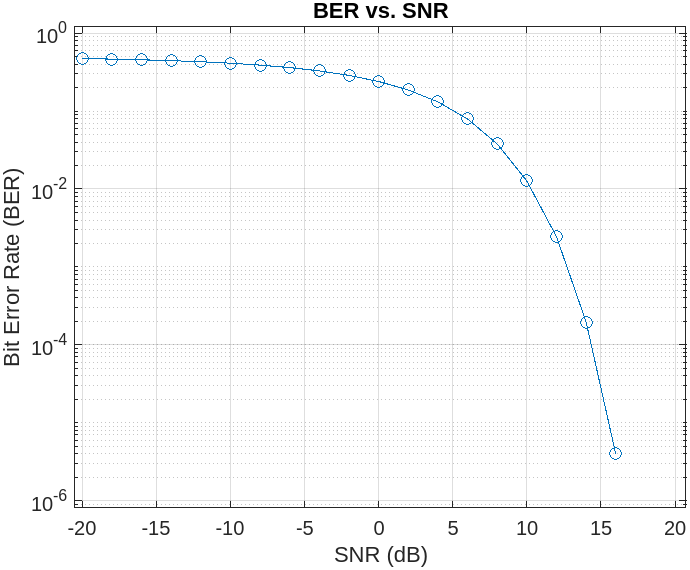
\includegraphics[width=0.51\textwidth]{lab_digital1.png}
			\caption{BER vs. SNR(dB)}
			\label{fig:plot}
		\end{figure}

\end{document}
